\section{Interface Design Description}
Dit hoofdstuk behandeld in detail alle interfaces en communicatie de het systeem
en daarmee subsystemen met elkaar hebben.

\subsection{Interface design}
\subsubsection{Drone interface}
De drone interface is wat de swarm aanroept om de fysieke drones, oftewel, de crazyflies, te besturen. De drone interface heeft verbinding met één bron en één gebruiker. De bron in dit geval, is het bestand 'tracking object.py', deze bron vertelt de drone interface waar de verbonden drone zich bevind in het speelveld. De gebruiker van de interface is het bestand 'swarm.py' waar alle commando's voor de swarm vandaankomen.
De verbinding tussen 'tracking object.py' en de drone interface, gebeurt doormiddel van mqtt berichten. 'tracking object.py' publiceerd de huidige locaties van fysieke drones op een kanaal genaamd 'drone', elke locatie krijgt het nummer van een drone mee: bv. drone 1, drone 2, enzovoort. De drone interface subscribed zich hieraan en krijgt zo zijn eigen locatie door de bijbehorende locatie van zijn eigen naam op te vragen. Dit gebeurt niet constant, maar er zit minder dan een seconde tussen de opvragen. 
De verbinding tussen 'swarm.py' en de drone interface, gebeurd via het importeren van de interface en hier per drone één instantie van te creëren. Deze drone interface instantie zal verantwoordelijk zijn voor het besturen van één van de drones en 'swarm.py' kan een specifieke instantie aanroepen om de bijbehorende drone een commando te geven. Dit gebeurd door direct de functies in de interface aan te roepen, wanneer dat nodig is. Er zit geen encryptie tussen de verschillende verbindingen, maar de mqtt server heeft een user, wachtwoord en adres.
\subsubsection{Simulation drone interface}
De simulation drone interface is wat de swarm aanroept om de gesimuleerde drones te besturen. De simulation drone interface heeft verbinding met één bron/ontvanger en één gebruiker. De bron/ontvanger in dit geval, is de applicatie webots, waarin de verschillende virtuele drones gesimuleerd worden. Webots vertelt de siulation drone interface waar de verbonden drone zich bevind op het virtuele speelveld. Ondertussen speelt webots hier ook als ontvanger, en krijgt van de simulation drone interface de commando's voor de bijbehorende drone door.
De verbinding tussen webots en de simulation drone interface gebeurt doormiddel van mqtt, de simulation drone interface publiceerd op het kanaal 'instructions' en subscribed aan het kanaal 'response', de locaties krijgen het nummer van een drone mee: vb. drone 0, drone 1, enzovoort. Op deze manier krijgt elke simulation drone interface zijn eigen locatie door, hier word een kleine delay ingestopt zodat het niet constant gebeurt, maar dit is minder dan een seconde.
De verbinding tussen 'swarm.py' en de simulation drone interface, gebeurd via het importeren van de interface en hier per drone één instantie van te creëren. Deze drone interface instantie zal verantwoordelijk zijn voor het besturen van één van de drones en 'swarm.py' kan een specifieke instantie aanroepen om de bijbehorende drone een commando te geven. Dit gebeurd door direct de functies in de interface aan te roepen, wanneer dat nodig is. Er zit geen encryptie tussen de verschillende verbindingen, maar de mqtt server heeft een user, wachtwoord en adres.

\subsection{Interface identification and diagrams}
\subsubsection{Drone interface}
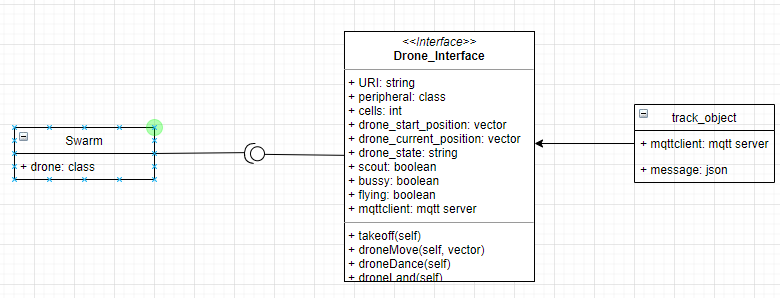
\includegraphics[width=\textwidth]{Latex/TECHDOCUMENT/drone_interface.PNG}
\subsubsection{Simulation drone interface}
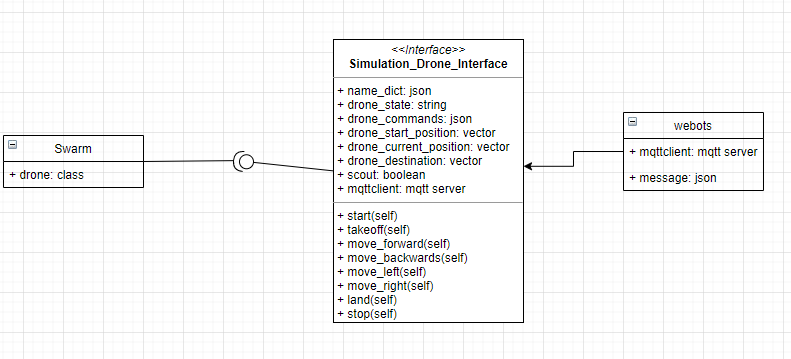
\includegraphics[width=\textwidth]{Latex/TECHDOCUMENT/simulation_drone_interface.PNG}

